%!TEX program = xelatex

\documentclass{article}
\usepackage[UTF8]{ctex}
\usepackage{indentfirst}
\usepackage{lmodern}% http://ctan.org/pkg/lm
\usepackage{setspace}
\usepackage{verbatim}
\usepackage{amsmath}
\usepackage{amsthm}
\usepackage{graphicx}
\usepackage{subfigure}
\usepackage{booktabs}
\usepackage{tabularx}
\usepackage{multirow}
\usepackage{multicol}
\usepackage{listings}
\usepackage{relsize}
\usepackage[usenames]{color}   
\usepackage{fontspec}

\usepackage[table]{xcolor}
\usepackage{array}
\usepackage[rightcaption]{sidecap}
\usepackage{hyperref}
\usepackage{float}
\usepackage{url}

% 自己画图
\usepackage{tikz}
\usepackage{mathpazo}
\usepackage{pgfplots}

% 插入动画
\usepackage{animate}
\usepackage{caption}
\usepackage{subfigure}
\usepackage{graphicx}

% 解决目录红框问题
\hypersetup{
colorlinks=true,
linkcolor=black
}

% 代码格式设置
\lstset{
         language = python, numbers=left, 
         numberstyle=\tiny,keywordstyle=\color{blue!70},
         commentstyle=\color{red!50!green!50!blue!50},frame=shadowbox,
         rulesepcolor=\color{red!20!green!20!blue!20},basicstyle=\ttfamily
}




\newcommand{\myd}{\;\mathrm{d}} %自定义积分变量命令
\renewcommand{\listtablename}{Tables} %改变listoftable的名字
\renewcommand{\arraystretch}{1.8} %行间距相对原始间距的倍数
% \setmonofont{Consolas}
\renewcommand\refname{参考网站}
% \setlength{\tabcolsep}{18pt} % 文本到单元格左右边框之间的距离
% \setlength{\arrayrulewidth}{0.4mm} % 设置表格线宽度


\setlength{\parindent}{2em} %控制首行缩进
\addtolength{\parskip}{3pt} %\parskip 控制段落(paragraph)距离
%\singlespacing % 设置单倍行距
%\doublespacing % 设置双倍行距
%\setstretch{1.25} % 设置行距为1.25
\onehalfspacing % 1.5倍行距
\graphicspath{{./figures/}} % 指定图片所在文件夹
%\newtheorem{definition}[定义]{section}
%定制环境: {环境名}[编号延续]{显示名}[编号层次]

%\begin{doublespacing} 特定行距环境 \end{doublespacing}


\begin{document}
\begin{titlepage}
% titlepage格式可以自己调
        \vspace*{-3cm}
	
	\begin{figure}[h]
		\centering
		
\includegraphics[width=0.7\linewidth]{zjdx}
	\end{figure}

	\vspace*{0.5cm}
	\begin{figure}[h]
		\centering
		
\includegraphics[width=0.5\linewidth]{QSY}
	\end{figure}
	\vspace{-0.5cm}
	\begin{center}
		\Huge{\textbf{应用光学实验}}\\
		
		\Huge{\textbf{实验报告}}
	\end{center}
	
	\vspace*{0.5cm}


	\vspace*{1cm}
    \begin{center}
            \Large 实验名称\ \ \underline{\makebox[220pt]{Title here}} \\ 
            \vspace{0.3cm}
            \quad \Large 姓名 \ \quad \underline{\makebox[220pt]{Peter H}} \\ 
            \vspace{0.3cm}
            \quad \Large 学号\ \quad \underline{\makebox[220pt]{3180xxxxxx}}\\
            \vspace{0.3cm}
            \Large 实验地点\ \ \underline{\makebox[220pt]{蓝田}}\\
            \vspace{0.3cm}
            \Large 实验日期\ \ \underline{\makebox[220pt]{2020年 mm 月 dd 日}}\\
            \vspace{0.3cm}
            \Large 指导老师\ \ \underline{\makebox[220pt]{Peter’s Instructors}}\\
            

             
    \end{center}
        
    
\end{titlepage}

\newpage
% \setcounter{tocdepth}{5}

\thispagestyle{empty} %清楚图片格式(取消掉编号)

% 不想要可以注释掉
\tableofcontents % 生成目录
\listoffigures%生成插图
\listoftables%生成表格
\thispagestyle{empty} 

\newpage
\pagenumbering{arabic}%重新开始标号,阿拉伯数字形式


\section{示例}
\subsection{图片示例}
\subsubsection{单一图片插入}
\begin{figure}[H]
\centering
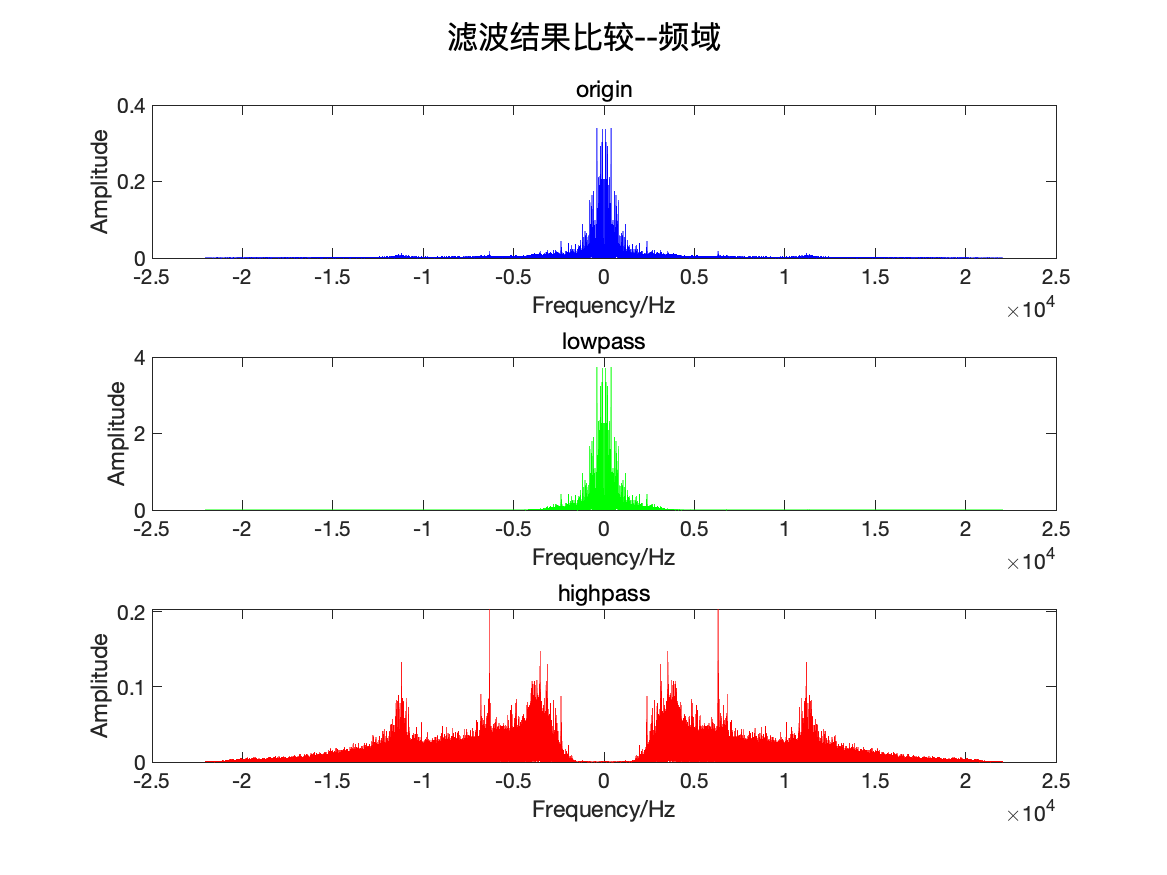
\includegraphics[width=0.8\textwidth]{filter-result-frequency}
\caption{来自声音处理的一个实验的酷酷的图片}
\end{figure}

\subsubsection{多图并入}
\begin{figure}[H]
% \subfigure 插入多图 计算好间距
\centering    
\subfigure[len-1] {    
\includegraphics[width=0.45\textwidth]{len3-1}  
}     
\subfigure[len-2] {     
\includegraphics[width=0.45\textwidth]{len3-2}     
}    
\subfigure[len-3] {    
\includegraphics[width=0.45\textwidth]{len3-3}  
}   
\subfigure[len-4] {    
\includegraphics[width=0.45\textwidth]{len3-4}  
}   

\caption{插入多图}  
      
\end{figure}



\subsection{表格示例}
\begin{table}[H]
  \centering
  \caption{数据记录表}
    \begin{tabular}{|c|c|c|}
    \hline
    \multicolumn{3}{|c|}{合并单元格}\\
    \hline
    \multicolumn{3}{|c|}{text}\\
    \hline
    手机焦距 $f_2'$/mm & 物到手机镜头的距离/mm &眼镜到手机的距离(透镜间隔 $d$/mm)\\
    \hline
    4.00  & 150.00  & 40.00  \\
    \hline
    像的放大倍率 $\beta$ &中间像到眼镜的位置/mm &中间像的大小$y'$/mm\\
    \hline
    0.024  & -63.25 & 5.75 \\
    \hline
    \end{tabular}
\end{table}

\subsection{代码示例}
\begin{lstlisting}
code here
set your language at line 48

\end{lstlisting}

\subsection{引用示例}
\begin{itemize}
 \item  LaTeX在线协作网站安利\cite{overleaf}
 \item  论文引用\cite{six-directional}
 \item  个人Blog安利嘿嘿\cite{myblog}

\end{itemize}

\subsection{动画示例}
\subsubsection{pdf插入动画的制作流程}

\begin{enumerate}
\item 手里有个gif
\item 在这里\cite{iloveimg}得到每一帧的图片
\item 改名,参考示例设置播放参数
\item 其他需求可自行搜索
\end{enumerate}

\subsubsection{Adobe Acrobat Needed}
需要用 Adobe Acrobat 打开pdf才能看到动态的动画,有些pdf阅读器不支持播放动画功能。
\begin{figure}[H]
\centering
\animategraphics[width=0.8\textwidth,autoplay=true,loop=true,controls=play]{5}{./6-inside/6-inside-00}{0}{24}
% controls = play 是只显示播放控件

\end{figure}


\subsection{Tikz示例}
\begin{figure}[H]
\centering
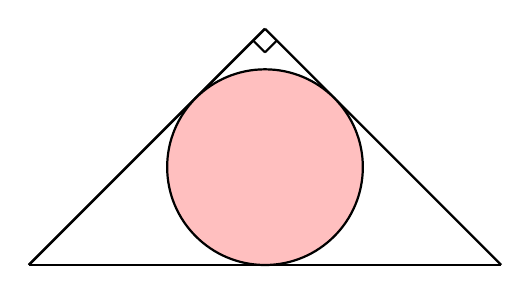
\begin{tikzpicture}[scale=3]
\draw [thick](-1,0)--(1,0);
\draw [thick](1,0)--(0,1);
\draw [thick](0,1)--(-1,0);
\draw [thick](-0.05,0.95)--(0,0.9);
\draw [thick](0,0.9)--(0.05,0.95);
\draw [thick](0,1)--(-1,0);
\draw [thick,fill=pink] (0,0.4142) circle(0.4142);
\end{tikzpicture}
\caption{画了个三角形内切圆}
\end{figure}



\newpage
% 参考网站
\begin{thebibliography}{9} %参考文献的数量
\bibitem{overleaf}
  \url{http://overleaf.com}

\bibitem{myblog}
  \url{http://longqianh.com}

\bibitem{iloveimg}
  \url{https://www.iloveimg.com/zh-cn/convert-to-jpg/gif-to-jpg }

\bibitem{six-directional}
Chen H, Zheng B, Shen L, et al. Ray-optics cloaking devices for large objects in incoherent natural light[J]. Nature communications, 2013, 4(1): 1-6.

\end{thebibliography}


\end{document}

